\documentclass[a4paper,12pt,openany]{book}
\usepackage [utf8]{inputenc}
\usepackage [french]{babel}
\usepackage [T1]{fontenc}
\usepackage{listings}
\usepackage{graphicx}
\usepackage{verbatim}

%%configuration de listings
\lstset{
language=c,
basicstyle=\ttfamily\small, 
identifierstyle=\color{red}, 
keywordstyle=\color{blue}, 
stringstyle=\color{black!60}, 
commentstyle=\it\color{green!95!yellow!1}, 
columns=flexible, 
tabsize=1, 
extendedchars=true, 
showspaces=false, 
showstringspaces=false, 
numbers=left, 
numberstyle=\tiny, 
breaklines=true, 
breakautoindent=true, 
captionpos=b
}

%coloration syntaxique
\usepackage{xcolor}
\definecolor{Zgris}{rgb}{0.87,0.85,0.85}

\newsavebox{\BBbox}
\newenvironment{DDbox}[1]{
\begin{lrbox}{\BBbox}\begin{minipage}{\linewidth}}
{\end{minipage}\end{lrbox}\noindent\colorbox{Zgris}{\\usebox{\BBbox}}
[.5cm]}

%Pour l espace entre la section et la chapitre (qui est trop grand).
\usepackage{titlesec}

\titleformat{\chapter}[block]
  {\normalfont\Huge\bfseries}% font of number
  {\chaptertitlename\ \thechapter~:}% format of number
  {20pt}% space between number and title
  {\Huge}% font of title

\titlespacing*{\chapter}
  {0pt}%  indent
  {0pt}% space before
  {20pt}% space after
\titlespacing*{\section}
  {0pt}%  indent
  {3.5ex plus 1ex minus .2ex}% space before
  {2.3ex plus .2ex}% space after

\author{Mendy Fatnassi}
\title{Cours de Programmation C}




%%%%%%%%%%%%%%%%%%%%%%%%%%%%%%%%%%%%%%	Page	%%%%%%%%%%%%%%%%%%%%%%%%%%%%%%%%%%%%%%%%

\begin{document}
\maketitle
\tableofcontents

\chapter{Arbre Binaire,N-aire,ARN,AVL}

\section{Generalité sur les Arbres}

En informatique un arbre est un ensemble de sommets organisé de facons hiéarchique tel qu'il existe un unique sommet appelé racine et qui n'a donc pas de superieure (père).\\
Tous les autres sommets sont atteints a partir de la racine par un unique chemins .\\
\\
De facons recursive (et constructive) un arbre est la donnée d'une racine et d'une liste d'arbres disjoints appelés sous-arbres.\\
Un sommet de l'arbre est la racine d'un sous-arbre.\\

\subsection{Principe}
Les arbres sont pratique pour la mise en place d'une structure de parcoure. Nous connaisons les structure de donnéé linéaire tels que les pile,file et liste maintenant nous allons voir des structure un peux plus complexe comme les arbres et les graphes (Cf.Cours_graphe).\\
\\
Les arbres, comme les listes, permettent de représenter un nombre variable de données. Le principal avantage des arbres par rapport aux listes est qu’ils permettent de ranger les données de telle sorte que les recherches soient plus efficaces.\\

\subsection{Définition}

-Un arbre est soit un noeud, soit un arbre vide.\\
\\
-Un noeud a des fils qui sont eux aussi des arbres.\\
\\
-Si tous les fils d’un noeud sont vides, alors le noeud est
qualifié de feuille.\\
\\
-Les noeuds portent des valeurs, ce sont les données que
l’on veut stocker.\\
\\
-Si tous les nœuds de l’arbre ont n fils, alors l’arbre est
dit n-aire.\\
\\
\underline{Exemple} : \\
\\
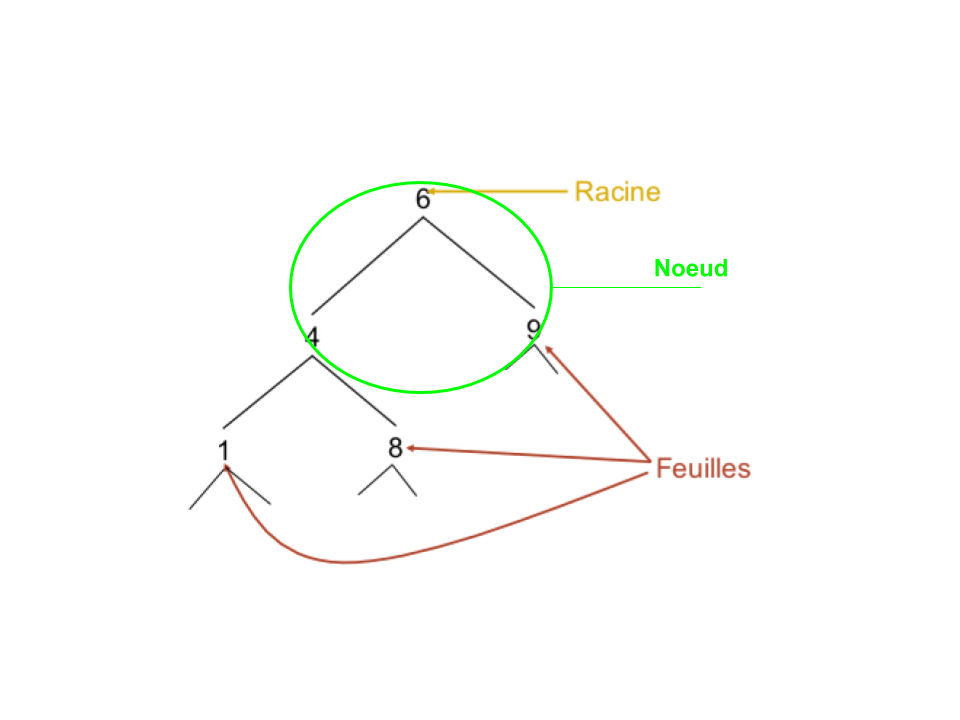
\includegraphics[width=1\linewidth,center]{img/definition_arbre.png}
\\
Un arbre d'un point de vie informatique et une structure de recherche ayant une valeur et 2 sous arbres (Gauche-Droit), mais en theorie des graphe,un arbre est un graphe non orienté connexe et sans cycle.\\

\susbsection{Terminologie}

Terminologie généalogique : \\
\\
-\textbf{père}: Prédécesseur d'un sommet.\\
-\textbf{fils}: Successeur d'un sommet.\\
-\textbf{frères}: Sommets qui ont le meme père.\\
On peut y ajouter les notions de (grand-père,descendants,etc.).\\
\\
\\
Terminologie forestière :\\
\\
-\textbf{racine}: Noeud qui ne possede pas de père.\\
-\textbf{feuilles}: Noeud (externes ou terminaux) qui n'ont pas de fils.\\
-\textbf{branches}: Généralement un chemin depuis un noeud racine (quelque fois jusqu'a une feuille).\\



\subsection{Mesures sur les Arbres}

La mesures sur les arbres sont tres utiles pour connaitre certainne caractéristique de l'arbre et permet aussi la mesure de la complexité des algorithmes sur les parcours d'arbres par exemple.\\

-\textbf{Profondeur}(Niveau) d'un noeud : Correspond a la longueur de la branche qui la joint a la racine (nombre d'arcs).\\
\\
-\textbf{Hauteur} d'un noeud: C'est la longueur de la plus longue branche de ce noeud jusqu'a une feuille.\\
\\
-\textbf{Hauteur} d'un arbre : C'est la longueur de la branche la plus longue (Hauteur de la racine).\\
\\
-\textbf{Taille} d'un arbre: Nombre de ses sommets.\\
\\
-\textbf{Longueur} totale : La somme des longueurs des branches issues de la racine.\\
\\
Voci un petit exemple :\\
\\
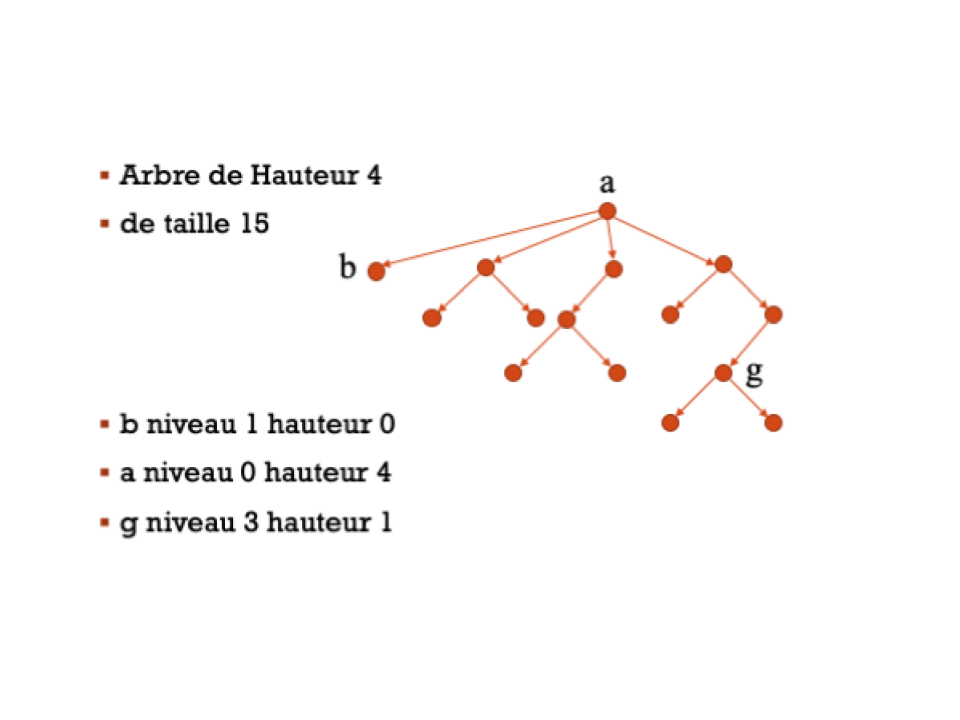
\includegraphics[width=1\linewidth,center]{img/exemple_mesure_arbre.png}
\\

%%%%%%%%%%%%%%%%%%%%%%%%%%%%%%%%%%%%%%%%%%%%%%%%%%%%%%%%%%%%%%%%%%%%%%%%%%%%%%%%%%%%%%%%%%%%%%%%%

\chapter{Parcours d'arbre}

\subsectin{Prefixe/Infixe/Postfixe}

Il s'agit de parcours en longueur , on va en voir 3 type :\\

Parcours Prefixe (Racine Gauche Droit): le noeud racine est traité au premier passage avant le parcours des sous-arbres .\\
\\
Parcours Infixe (ou Symetrique) (Gauche Racine Droit): On commenca par examiner le noeud gauche puis la racine et on finipar sson noeud droit.\\
\\
Parcours Postfixe (Gauche Droit Racine): Meme principe.\\

\subsection{Largeur}

Le parcours en largeur , consiste a traiter chaque noeud de gauche a droite sur chque ligne de l'arbre.\\



%%%%%%%%%%%%%%%%%%%%%%%%%%%%%%%%%%%%%%%%%%%%%%%%%%%%%%%%%%%%%%%%%%%%%%%%%%%%%%%%%%%%%%%%%%%%%%%%%

\chapter{Arbre Binaire}

-Arbre binaire complet: Chaque noeud a 0 ou 2 fils .\\
-Arbre binaire parfait: Arbre complet + Toutes les feuilles sont a la meme hauteur.\\
-Arbre binaire quasi-parfait: Arbre parfait sauf qu'il peux manqué des feuilles a droite.\\

Un arbre binaire est :\\
\\
-soit l’arbre vide\\
-soit un noeud qui a exactement deux fils (éventuellement vides)\\
\\ 
Pour manipuler les arbres binaires, on a besoin de primitives d’\textbf{accès} : \\
\textbf{valeur} : retourne la valeur d’un arbre non vide\\
\textbf{fils-g} : retourne le fils de gauche d’un arbre non vide\\
\textbf{fils-d} : retourne le fils de droite d’un arbre non vide\\
\\
de primitives de \textbf{test} :\\
\textbf{vide}? : retourne vrai si un arbre donné est vide\\
\textbf{arbre}=? : retourne vrai si deux arbres donnés sont égaux\\

de primitives de \textbf{construction} :\\
\textbf{creerArbre} : retourne un arbre vide\\
\textbf{cons-binaire} : crée un arbre avec une valeur donnée et deux arbres donnés qui seront ses deux uniques fils .\\

\section{Implementation par tas}

Implementation par tas d'un arbre.\\

typedef enum tas_type{MIN,MAX} t_tas_type;

typedef struct tas{
  int *tas;
  int nb_val,nc,max_val;
  t_tas_type type;
}t_tas;

typedef struct tas * t_tas;

\subsection{Primitive}

/*****Primitive de Creation*****/
t_tas creer_tas (int nbv){
  t_tas * t=malloc(sizeof(t_tas));
  t->tas=malloc(sizeof(int)*nbv);
  t->nb_val=0;
  return t;
}


-Pour trouvé un fils gauche(fg) ou un fils droite(fd) dans un arbre qui est representer par un tableau on peux appliquer les formule suivante :\\
fg=2n+1 et fd=2n+2 (ou n est le numeros du noeud a l'indice i)\\
\\
\underline{Exemple}:\\
\\
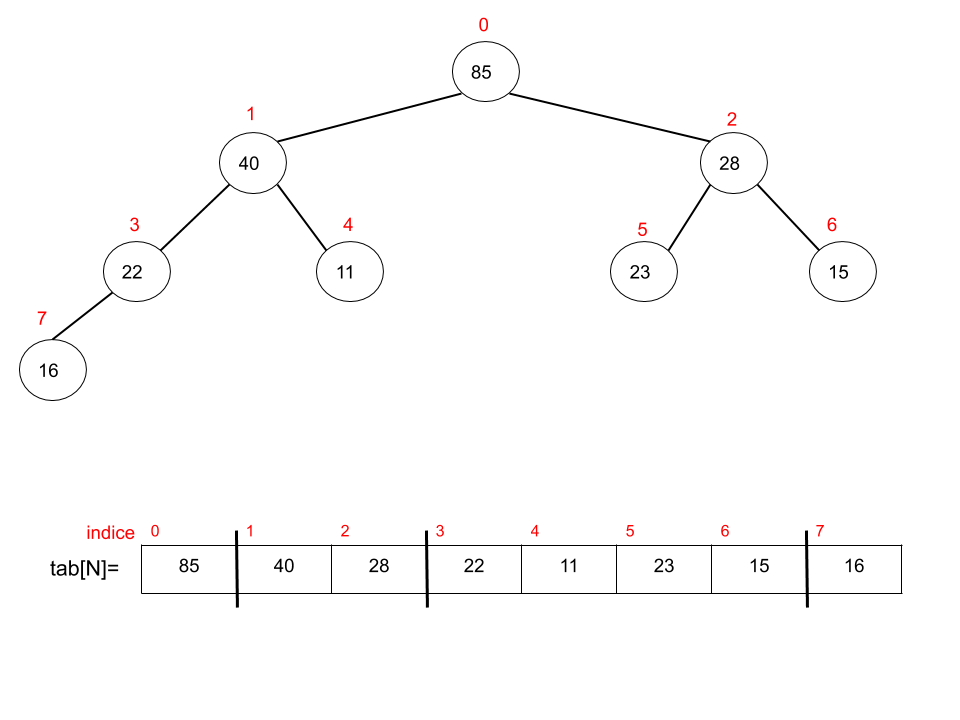
\includegraphics[width=1\linewidth,center]{img/arbre_impl_tab.png}


/*****Primitive de Test*****/



%%%%%%%%%%%%%%%%%%%%%%%%%%%%%%%%%%%%%%%%%%%%%%%%%%%%%%%%%%%%%%%%%%%%%%%%%%%%%%%%%%%%%%%%%%%%%%%%%

\chapter{Arbre ARN}

%%%%%%%%%%%%%%%%%%%%%%%%%%%%%%%%%%%%%%%%%%%%%%%%%%%%%%%%%%%%%%%%%%%%%%%%%%%%%%%%%%%%%%%%%%%%%%%%%

\chapter{Arbre N-aire}



\end{document}